\chapter{Pruebas y Resultados Preliminares}
En este capítulo veremos los resultados de la pruebas llevadas a cabo con diferentes algoritmos.
\section{Efectos del pre-procesamiento}
En esta sección presentamos la realización de un experimento para determinar el efecto de los métodos de pre-procesamiento, el objetivo es observar los porcentajes de reconocimiento para varias configuraciones de pre-procesamiento en \ac{PCA} en su entrenamiento así como en el momento de reconocimiento.
Para ello el desarrollo de las pruebas fue el siguiente:
\begin{itemize}
\item Se seleccionaron diez sujeto de cada base de datos, en el caso de la base de datos de AT \& T hay diez imágenes por sujeto y en la base de datos de Yale ya once. Se tomó una imagen mirando de frente por sujeto, para el entrenamiento y el resto para realizar pruebas de reconocimiento.
\item Para las pruebas de reconocimiento y entrenamiento se eligieron los siguientes opciones de pre-procesamientos, ya explicados: sin pre-procesamiento alguno, ecualización del histograma, ecualización adaptativa del histograma con una vecindad de 2 y 4 pixeles, procesos de binarización con mascara de media y con mascara gaussiana, finalmente el canal Parvocelular del modelo retina.
\item Se elige una opción antes mencionada para aplicar a las imágenes destinadas al entrenamiento, después de ello se el aplica a las imágenes de prueba las opciones de pre-procesamiento una la vez, y se procede a realizar el reconocimiento, anotando los porcentaje de acierto, una vez realizada las pruebas con todas las opciones se vuelve a entrenar el reconocimiento con la siguiente opción de pre-procesamiento hasta usar todas las combinaciones.
\end{itemize}
\begin{figure}[h]
    \center
    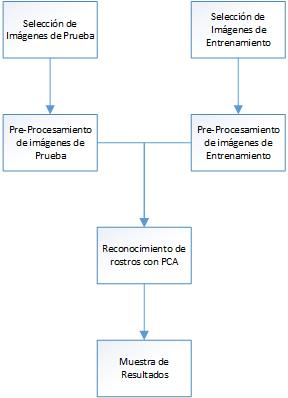
\includegraphics[scale=0.6]{Esquema.jpg}
    \caption{Esquema de realización de Pruebas.}
\end{figure}
\subsection{Resultados}
En la figura 6 se puede apreciar el proceso de por el cual se obtuvieron los resultados que fueron traducidos en las tablas 2 y 3 para poder ser interpretados con mayor facilidad.
\subsection{Base de datos AT \& T}
Es una base de datos de diez imágenes diferentes por cada uno de los 40 de las diferentes personas. En algunos sujetos, las imágenes fueron tomadas en diferentes momentos, variación de iluminación, expresiones faciales (ojos abiertos / cerrados, sonriendo / No sonrientes) y los detalles faciales (gafas / sin gafas). Todas las imágenes fueron tomadas contra un fondo oscuro homogéneo con los sujetos en posición vertical, frontal (con tolerancia para un cierto movimiento lateral).
\begin{figure}[h]
    \center
    \includegraphics[scale=0.2]{att}
    \caption{Ejemplo de la base de datos de AT \& T.}
\end{figure}
Según los datos mostrados en la tabla 2 podemos hacer las siguientes observaciones:
\begin{itemize}
\item Vemos una clara tendencia a una mayor cantidad de aciertos cuando la imagen es sujeta a el mismo pre-procesamiento en el entrenamiento como en el  prueba de reconocimiento, cabe resaltar que las combinaciones con mayor cantidad de aciertos son cuando se entrena y se prueba sin pre-procesamiento y con el canal Parvocelular del modelo retina.
\item En el caso de los entrenamientos con mascaras de binarización los resultados son siempre cero, eso puede explicarse que a pesar de eliminar contraste, el proceso de binarización en sí no es apto para tareas de reconocimiento con \ac{PCA} debido a que al transformar los datos a un vector de pesos solo se acumulan en los valores cero y 255 de la escala de grises lo cual no importando la forma de la figura si tiene la misma cantidad de pixeles blancos y negros, no podrán diferenciarse de otras imágenes.
\item El entrenamiento con ecualización del histograma y las pruebas con \ac{CLAHE} presentan cero por ciento de aciertos, esto puede explicarse ya que a pesar de ser ambas ecualizaciones \ac{CLAHE} trabaja por vecindades lo que evita la amplificación del ruido en grandes áreas a diferencia del proceso normal de ecualización lo que genera diferencias al momento del calculo de valores de \ac{PCA}.
\item La mayoría de las combinaciones no llegan al 70\% de aciertos lo que resalta la sensibilidad a variaciones de luz que posee \ac{PCA}, por ser un método estadístico de reconocimiento.
\end{itemize}
\begin{table}%[h]
\resizebox{\columnwidth}{13mm}{
\begin{tabular}{|c|c|c|c|c|c|c|c|}
\hline
\textbf{Prueba/Entrenamiento}  & \textbf{Sin pre-procesamiento} & \textbf{Ecualización de hist.} & \textbf{CLAHE (vecindad 2)} & \textbf{CLAHE (vecindad 4)} & \textbf{Binarización media} & \textbf{Binarización gaussiana} & \textbf{Parvocelular} \\ \hline
\textbf{Sin pre-procesamiento} &            88.8\%              &            27.7\%              &           0\%               &           0\%               &          0\%          &     0\%   &      0\%              \\ \hline
\textbf{Ecualización de hist.} &           74.4\%               &            53.3\%              &          6.6\%              &         7.7\%               &          0\%          &    0\%    &      0\%              \\ \hline
\textbf{CLAHE (vecindad 2)}    &             0\%                &           40\%                 &          73.3\%             &         64.4\%              &          0\%          &    0\%    &      75.5\%            \\ \hline
\textbf{CLAHE (vecindad 4)}    &             0\%                &            27.7\%              &          68.8\%             &         65.5\%              &          0\%          &    0\%    &      66.6\%            \\ \hline
\textbf{Binarización media}    &             3.3\%              &            23.3\%              &          40\%               &          44.4\%             &          0\%          &    0\%    &     65.5\%           \\ \hline
\textbf{Binarización gaussiana}&              14.4\%            &          36.6\%                &          43.3\%             &          51.1\%             &           0\%         &    0\%    &      12.2\%             \\ \hline
\textbf{Parvocelular}           &             0\%                &           4.4\%                &           18.8\%            &          15.5\%             &           0\%         &    0\%    &      82.2\%             \\ \hline
\end{tabular}
}
\caption{Porcentaje de aciertos con la Base de datos AT \& T}
\end{table}
\subsection{Base de datos Yale}
Contiene 165 imágenes en escala de grises en formato GIF de 15 individuos. Hay 11 imágenes por sujeto, una por expresión facial diferente o configuración: centro-luz, con gafas, feliz, iluminación izquierda, sin gafas, normal, iluminación derecha, triste, soñoliento, sorprendido,y guiño.
\begin{figure}[h]
    \center
    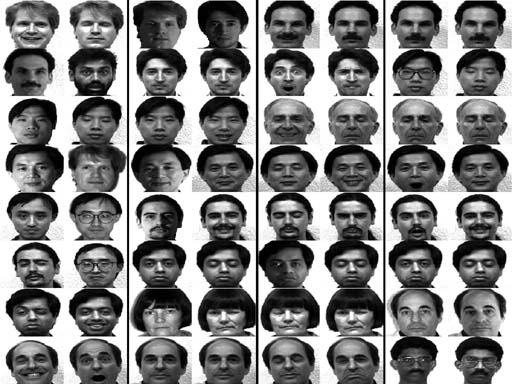
\includegraphics[scale=0.8]{yalefaces}
    \caption{Ejemplo de la base de datos de Yale.}
\end{figure}
En el caso de la base de datos Yale y sus resultados en la tabla 3.
\begin{itemize}
\item Como se aprecia en el caso anterior la binarización para el en tratamiento de \ac{PCA} no es efectiva.
\item Aquí es menor la tasa de aciertos a comparación a la anterior base de datos, esto puede explicarse por la naturaleza de las fotografías, mientras en la base de datos de AT \& T existían variaciones de expresión facial, ligeros cambios de pose, también existía leves cambios de iluminación a comparación de los que presenta esta base de datos, que se enfoca en diferentes fuentes de iluminación.
\item La configuración con mayor porcentaje de aciertos es un entrenamiento y pruebas si pre-procesamiento, lo que pude indicar que en condiciones de iluminación drásticas los pre-procesamientos que mejoran detalles y contraste, a pesar que mejora la visualización de la imagen, para el proceso de \ac{PCA} eliminan información importante.
\end{itemize}
\begin{table}%[h]
\resizebox{\columnwidth}{13mm}{
\begin{tabular}{|c|c|c|c|c|c|c|c|}
\hline
\textbf{Prueba/Entrenamiento}  & \textbf{Sin pre-procesamiento} & \textbf{Ecualización de hist.} & \textbf{CLAHE (vecindad 2)} & \textbf{CLAHE (vecindad 4)} & \textbf{Binarización media} & \textbf{Binarización gaussiana} & \textbf{Parvocelular} \\ \hline
\textbf{Sin pre-procesamiento} &             35\%               &          7\%                   &               0\%           &            0\%              &         0\%           &   0\%     &     0\%               \\ \hline
\textbf{Ecualización de hist.} &             1\%                &           26\%                 &               27\%          &            6\%              &         0\%           &   0\%     &     0\%               \\ \hline
\textbf{CLAHE (vecindad 2)}    &            21\%                &           5\%                  &              2\%            &            7\%              &        0\%            &   0\%     &     0\%               \\ \hline
\textbf{CLAHE (vecindad 4)}    &            7\%                 &           0\%                  &              29\%           &            24\%             &         0\%           &   0\%     &     0\%               \\ \hline
\textbf{Binarización media}    &             0\%                &           0\%                  &             27\%            &            26\%             &         0\%           &   0\%     &      0\%              \\ \hline
\textbf{Binarización gaussiana}&              0\%               &           0\%                  &              0\%            &            0\%              &         7\%           &    0\%    &     11\%              \\ \hline
\textbf{Parvocelular}           &              0\%               &           0\%                  &             4\%             &            4\%              &         0\%           &    7\%    &      6\%              \\ \hline
\end{tabular}
}
\caption{Porcentaje de aciertos con la Base de datos Yale}
\end{table}

\subsection{Conclusión sobre el experimento}
Para finalizar presentamos nuestras conclusiones:
\begin{itemize}
\item Un método de reconocimiento estadístico como lo es \ac{PCA} tiene un gran funcionamiento cuando las condiciones de iluminación son controladas, como se pudo apreciar en las dos base de datos, \ac{PCA} puede lograr un buenas tazas de reconocimiento con pequeñas variaciones en posición del rostro y expresión facial.
\item En el caso de ambientes no controlados, donde los ángulos de visión, la iluminación y las expresiones faciales varían en gran medida es recomendable y un método que no sea estadístico como \ac{PCA} ya que es sensible a dichas variaciones.
\item Para el caso de ambientes no controlados se aconseja probar con métodos de reconocimientos que estén basados en la biométrica de los rostros.
\item Para que muchos de los métodos de  reconocimiento actuales  puedan funcionar de manera correcta es siempre necesaria la colaboración del las personas a identificar, pero es necesario buscar formas de reconocimiento sin la cooperación de las personas
%\item A pesar de que existen muchas areas donde el reconocimiento en la vida real es posible, aun queda muchos contextos donde se necesita mayor investigación tal como las cámaras de seguridad.
\item El pre-procesamiento es una parte importante del reconocimiento de rostros pero es necesario entender a profundidad la naturaleza del método de reconocimiento para poder elegir el pre-procesamiento adecuado.
\item Para el caso de \ac{PCA} podemos concluir que los pre-procesamiento que mejoran el contraste e imágenes con la iluminación adecuada son los más adecuados para alcanzar altas tasas de de reconocimiento.
\end{itemize}

\section{Pruebas del detector de rostros}
Para determinar los efectos del pre-procesamiento en el desempeño del detector de rostros se realizaron pruebas con un conjunto de entrenamiento de imágenes de rostros frontales y usando la base de datos conocida como \textit{Face in the wild}, que consiste en fotografías tomadas de los medios de prensa en diversas situaciones y en ambientes no controlados.
\begin{figure}[h]
    \center
    \includegraphics[scale=0.3]{FaceInTheWild.PNG}
    \caption{Ejemplo de la base de datos Face in the Wild}
\end{figure}

Las pruebas se realizaron con cincuenta imágenes tomadas al azar las cuales contenían diferentes números de rostros por imagen pero dando un total de cien rostros, el cuadro de resultados contiene el numero de detecciones, incluyendo las detecciones acertadas y los falso positivos, para los caso de pre-procesamiento vistos en la prueba anterior.
\begin{table}[th]
%\label{my-label}
\resizebox{\columnwidth}{13mm}{
\begin{tabular}{|l|c|c|c|c|c|c|c|}
\hline
{\bf \begin{tabular}[c]{@{}l@{}}Método de\\ pre-procesamiento\end{tabular}} & {\bf Sin pre-procesamiento} & {\bf Ecualización de histograma} & {\bf CLAHE (vecindad 2)} & {\bf CLAHE (vecindad 4)} & {\bf Binarización media} & {\bf Binarización Gausiana} & {\bf \begin{tabular}[c]{@{}c@{}}Modelo retina:\\ Parvocelular\end{tabular}} \\ \hline
{\bf Nro  de rostros}                                                       & 100                         & 100                              & 100                      & 100                      & 100                      & 100                         & 100                                                                         \\ \hline
{\bf Rostros detectados}                                                    & 88                          & 88                               & 88                       & 81                       & 15                       & 16                          & 96                                                                          \\ \hline
{\bf rostros correctamente detectados}                                      & 82                          & 84                               & 81                       & 78                       & 15                       & 16                          & 84                                                                          \\ \hline
{\bf Falsos positivos}                                                      & 6                           & 4                                & 7                        & 3                        & 0                        & 0                           & 12                                                                          \\ \hline
\end{tabular}
}
\centering
\caption{Resultados de la prueba del detector de Viola-jones con imágenes de rostros frontales como entrenamiento}
\end{table}